\documentclass[11pt]{opticajnl}
\journal{opticajournal} % use for journal or Optica Open submissions

% See template introduction for guidance on setting shortarticle option
\setboolean{shortarticle}{true}
% true = letter/tutorial
% false = research/review article

% ONLY applicable for journal submission shortarticle types:
% When \setboolean{shortarticle}{true}
% then \setboolean{memo}{true} will print "Memorandum" on title page header
% Otherwise header will remain as "Letter"
% \setboolean{memo}{true}
\usepackage{lineno}
\usepackage{listings}
\usepackage{xcolor}  % Para colorear el código

% Definir colores para la sintaxis de Python
\definecolor{pystring}{RGB}{186,33,33}      % Strings
\definecolor{pycomment}{RGB}{107,107,107}   % Comentarios
\definecolor{pykeyword}{RGB}{0,119,170}     % Palabras clave
\definecolor{pybuiltin}{RGB}{163,21,21}     % Funciones builtin
\definecolor{pybackground}{RGB}{250,250,250} % Fondo

% Definir el estilo para código Python
\lstdefinestyle{Python}{
    language=Python,
    backgroundcolor=\color{pybackground},
    basicstyle=\ttfamily\small,
    breakatwhitespace=false,
    breaklines=true,
    captionpos=b,
    keepspaces=true,
    numbers=left,
    numbersep=5pt,
    showspaces=false,
    showstringspaces=false,
    showtabs=false,
    tabsize=4,
    frame=single,
    commentstyle=\color{pycomment},
    keywordstyle=\color{pykeyword},
    stringstyle=\color{pystring},
    identifierstyle=\color{black},
    numberstyle=\tiny\color{gray},
    emphstyle=\color{pybuiltin},
    morekeywords={import,from,as,def,class,return,yield,for,while,if,else,elif,
                  try,except,finally,with,lambda,assert,pass,break,continue,
                  raise,global,nonlocal,True,False,None,and,or,not,is,in},
    emph={pandas,numpy,matplotlib,seaborn,sklearn,tensorflow,torch,
          plt,pd,np,sns,print,len,range,enumerate,zip,dict,list,tuple,set,
          min,max,sum,sorted,map,filter},
}

\lstdefinestyle{sql}{
  language=SQL,
  showspaces=false, 
  basicstyle=\ttfamily,
  numbers=left,
  numberstyle=\tiny,
  backgroundcolor=\color{gray!10},
  keywordstyle=\color{blue}\bfseries,
  commentstyle=\color{green!70}\ttfamily,
  stringstyle=\color{red!70}\ttfamily,
  breaklines=true,
  morekeywords={CREATE, DROP, TABLE, SELECT, INSERT, UPDATE, DELETE, FROM, WHERE, JOIN, ON, AS}, % Puedes añadir más palabras clave específicas de SQL.
  literate={``}{``}1 {''}{''}1 {“}{``}1 {”}{''}1 {‘}{`}1 {’}{'}1
}

\lstdefinestyle{terminal}{
  backgroundcolor=\color{white},   % Fondo blanco
  basicstyle=\color{black}\ttfamily, % Texto negro en fuente monoespaciada
  keywordstyle=\color{blue}\bfseries, % Palabras clave en azul y negrita
  commentstyle=\color{green!70}\ttfamily, % Comentarios en verde
  stringstyle=\color{red}\ttfamily, % Cadenas en rojo
  morekeywords={sudo, apt-get, install, cd, ls, mkdir, rm, rmdir, cp, mv, echo, cat, nano, vim, grep, find, chmod, chown, systemctl, service, update, upgrade, reboot, shutdown, exit}, % Comandos comunes de terminal
  breaklines=true, % Permitir saltos de línea
  frame=single, % Marco alrededor del código
  framerule=0.5pt, % Grosor del marco
  rulecolor=\color{gray}, % Color del marco
  xleftmargin=0.05\textwidth, % Margen izquierdo
  xrightmargin=0.05\textwidth, % Margen derecho
  aboveskip=1em, % Espacio antes del bloque de código
  belowskip=1em % Espacio después del bloque de código
}
\definecolor{rstring}{RGB}{186,33,33}     % Strings
\definecolor{rcomment}{RGB}{0,128,0}      % Comentarios
\definecolor{rfunction}{RGB}{0,0,255}      % Funciones
\definecolor{rkeyword}{RGB}{145,0,145}    % Palabras clave
\definecolor{rbackground}{RGB}{248,248,248} % Fondo

\lstdefinestyle{R}{
    language=R,
    backgroundcolor=\color{rbackground},
    basicstyle=\ttfamily\small,
    breakatwhitespace=false,
    breaklines=true,
    captionpos=b,
    keepspaces=true,
    numbers=left,
    numbersep=5pt,
    showspaces=false,
    showstringspaces=false,
    showtabs=false,
    tabsize=2,
    frame=single,
    commentstyle=\color{rcomment},
    keywordstyle=\color{rkeyword},
    stringstyle=\color{rstring},
    identifierstyle=\color{black},
    numberstyle=\tiny\color{gray},
    morekeywords={library, data.frame, read.csv, ggplot, aes, geom_bar, theme_minimal, 
                  scale_fill_manual, gather, group_by, summarise, arrange, filter},
}


%\linenumbers % Turn off line numbering for Optica Open preprint submissions.

\title{Consultas MDX}

\author[1,2,3]{Luis Ardévol Mesa}


\begin{abstract}
El objetivo de esta práctica es realizar 5 consultas MDX sobre los datos de finanzas o satisfacción de usuarios de nuestra base de datos. Se describen las consultas realizadas, acompañadas de los resultados y el código MDX correspondiente.
\end{abstract}

\setboolean{displaycopyright}{false} % Do not include copyright or licensing information in submission.

\begin{document}

\maketitle

En caso de no copiarse correctamente el código MDX, se pueden encontrar las consultas en el archivo \texttt{README} adjunto.

\section{Identificar las combinaciones de director y productor con mayor rentabilidad, calculando el retorno de inversión (ROI) promedio de sus proyectos, mostrando solo el top 30.}

\subsection{Descripción}

El ROI se calcula como 
\begin{equation*}
\text{ROI} = \frac{\text{ingresos} - \text{coste}}{\text{coste}} = \frac{\text{beneficio}}{\text{coste}}
\end{equation*}

Esta consulta permite identificar de forma rápida combinaciones que generan grandes retornos de inversión, lo cual es importante para las productoras, al identificar colaboraciones rentables (o con expectativas de serlo). \\

Para hacerla en Saiku, se crea el ROI como medida calculada, se seleccionan los productores y directores para las filas de la representación y el ROI como medida, y se limita a un top 30 ordenado por ROI.

\subsection{Código MDX generado}
\begin{lstlisting}[style=terminal]
WITH
MEMBER [Measures].[roiPromedio] AS
	(([Measures].[beneficio]) / [Measures].[coste])
SET [~ROWS_productor_productor.jerarquiaproductor] AS
	{[productor.jerarquiaproductor].[nivelproductor].Members}
SET [~ROWS_director_director.jerarquiadirector] AS
	{[director.jerarquiadirector].[niveldirector].Members}
SELECT
NON EMPTY {[Measures].[roiPromedio]} ON COLUMNS,
NON EMPTY Order(TopCount(NonEmptyCrossJoin([~ROWS_productor_productor.jerarquiaproductor], [~ROWS_director_director.jerarquiadirector]), 30, ([Measures].[beneficio] / [Measures].[coste])), [Measures].[beneficio]/[Measures].[coste], DESC) ON ROWS
FROM [finanzas]
\end{lstlisting}

\newpage
\subsection{Resultado}
\begin{figure}[h]
\centering
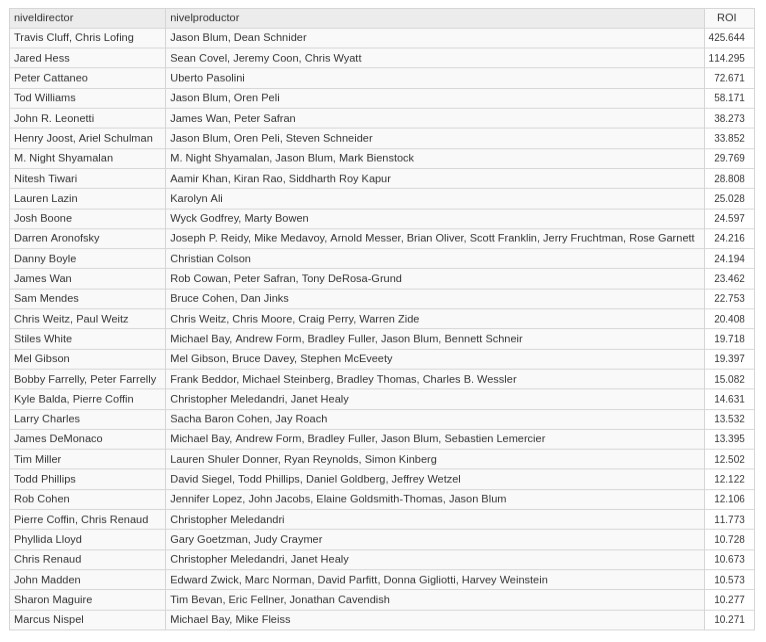
\includegraphics[width=0.8\textwidth]{fotos/con1.jpg}
\caption{Resultado de la consulta 1.}
\end{figure}


\newpage

\section{Determina la tendencia de ingresos por productora a partir de la diferencia entre los ingresos actuales y los ingresos del año anterior}

\subsection{Descripción}

Esta consulta ayuda a evaluar cómo evolucionaron sus ingresos en el último año, lo que permite tomar decisiones para mejorar o mantener sus actividades actuales. \\

Para hacer esta consulta en Saiku, se crea una medida calculada llamada tendencia, que calcula la diferencia entre los ingresos actuales y los del año anterior. Se seleccionan las productoras para las filas y la tendencia como medida.

\subsection{Código MDX generado}

\begin{lstlisting}[style=terminal]
WITH
MEMBER [Measures].[tendencia] AS
	(([tiempoemision].[anno].CurrentMember, [Measures].[ingresos]) - [tiempoemision].[anno].PrevMembe)
SET [~ROWS] AS
	Order({[productora.jerarquiaproductora].[nivelproductora].Members}, ([tiempoemision].[anno].CurrentMember, [Measures].[ingresos]) - [tiempoemision].[anno].PrevMembe, [Measures].[ingresos], ASC)
SELECT
NON EMPTY {[Measures].[tendencia]} ON COLUMNS,
NON EMPTY [~ROWS] ON ROWS
FROM [finanzas]
\end{lstlisting}

\subsection{Resultado}

\begin{figure}[h]
\centering
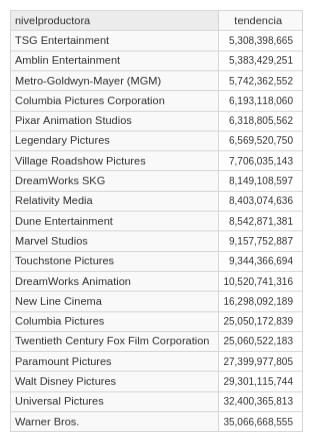
\includegraphics[width=0.3\textwidth]{fotos/con2.jpg}
\caption{Resultado de la consulta 2.}
\end{figure}

\newpage

\section{Comparar el porcentaje de mercado en ingresos de cada productora por año. Muestra los mejores porcentajes de los últimos 20 años.}

\subsection{Descripción}

Esta consulta es esencialmente mostrar la cuota de mercado de cada productora en términos de sus ingresos. Esto es de utilidad para que las productoras conozcan su posición en el mercado actual y puedan tomar decisiones estratégicas en consecuencia. \\

Para hacer esta consulta en Saiku, se crea una medida calculada llamada cuota de mercado, que calcula el porcentaje de ingresos de cada productora en relación con el total de ingresos de la industria (otra medida calculada). Se seleccionan las productoras y los años para las filas y la cuota de mercado como medida. Se limita a los 10 mejores porcentajes de los últimos 20 años.

\subsection{Código MDX generado}

\begin{lstlisting}[style=terminal]
WITH
MEMBER [Measures].[cuotaMercado] AS
	((100 * [Measures].[ingresos]) / Sum([productora].[nivelproductora].Members, [Measures].[ingresos]))
SET [~ROWS_productora_productora.jerarquiaproductora] AS
	{[productora.jerarquiaproductora].[nivelproductora].Members}
SET [~ROWS_tiempoemision_tiempoemision.jerarquiatiempo] AS
	{[tiempoemision.jerarquiatiempo].[anno].Members}
SELECT
NON EMPTY {[Measures].[cuotaMercado]} ON COLUMNS,
NON EMPTY TopCount(NonEmptyCrossJoin([~ROWS_productora_productora.jerarquiaproductora], [~ROWS_tiempoemision_tiempoemision.jerarquiatiempo]), 10, [Measures].[ingresos]) ON ROWS
FROM [finanzas]
\end{lstlisting}

\subsection{Resultado}

\begin{figure}[h]
\centering
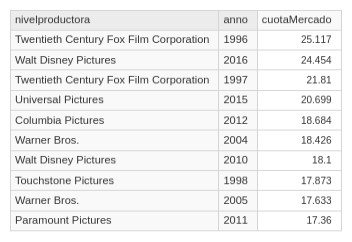
\includegraphics[width=0.45\textwidth]{fotos/con3.jpg}
\caption{Resultado de la consulta 3.}
\end{figure}

\newpage

\section{Identifica los ingresos de las productoras cada año. Muestra los años con mayores ingresos.}

\subsection{Descripción}

Esta consulta es de utilidad para que las productoras conozcan su desempeño financiero a lo largo del tiempo, lo que les permite identificar tendencias y ver cómo la toma de decisiones ha ido influyendo en sus ingresos. \\

Para hacer esta consulta en Saiku, se seleccionan los años y las productoras para las filas y los ingresos como medida. Se limita a los años con mayores ingresos de cada productora.

\subsection{Resultado}

\begin{figure}[h]
\centering
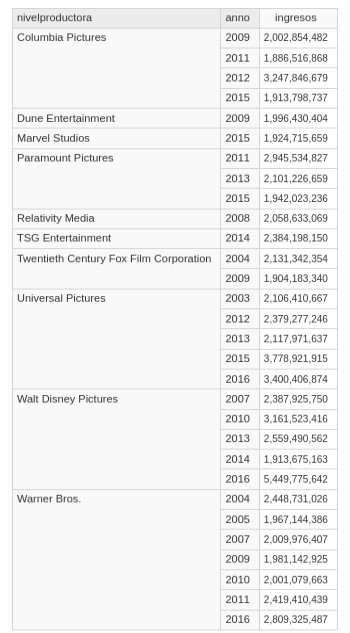
\includegraphics[width=0.5\textwidth]{fotos/con4.jpg}
\caption{Resultado de la consulta 4.}
\end{figure}

\subsection{Código MDX generado}

\begin{lstlisting}[style=terminal] 
WITH
SET [~ROWS_productora_productora.jerarquiaproductora] AS
	{[productora.jerarquiaproductora].[nivelproductora].Members}
SET [~ROWS_tiempoemision_tiempoemision.jerarquiatiempo] AS
	{[tiempoemision.jerarquiatiempo].[anno].Members}
SELECT
NON EMPTY {[Measures].[ingresos]} ON COLUMNS,
NON EMPTY Order(TopCount(NonEmptyCrossJoin([~ROWS_productora_productora.jerarquiaproductora], [~ROWS_tiempoemision_tiempoemision.jerarquiatiempo]), 30, [Measures].[ingresos]), [productora.jerarquiaproductora].[nivelproductora].CURRENTMEMBER.ORDERKEY, ASC) ON ROWS
FROM [finanzas]
\end{lstlisting}


\newpage


\section{Evaluar el impacto de los costos en los ingresos de cada director. Muestra los 20 directores con mayores beneficios.}

\subsection{Descripción}

Esta consulta es útil para analizar si mayores costos se correlacionan con mayores ingresos para cada director. También ayuda a identificar directores que han logrado mantener altos ingresos a pesar de los costos, lo que puede ser útil para producciones de menor presupuesto que quieran mantener altos beneficios. \\

Para hacer esta consulta en Saiku, se seleccionan los directores para las filas y los ingresos, los costos y los beneficios como medidas. Se limita a los directores con mayores beneficios.

\subsection{Resultado}

\begin{figure}[h]
\centering
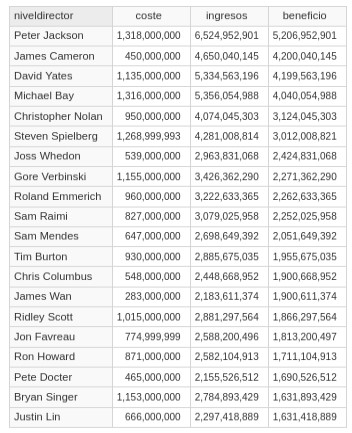
\includegraphics[width=0.48\textwidth]{fotos/con5.jpg}
\caption{Resultado de la consulta 5.}
\end{figure}

\subsection{Código MDX generado}

\begin{lstlisting}[style=terminal]
WITH
SET [~ROWS] AS
	Order(TopCount({[director.jerarquiadirector].[niveldirector].Members}, 20, [Measures].[beneficio]), [Measures].[beneficio], DESC)
SELECT
NON EMPTY {[Measures].[coste], [Measures].[ingresos], [Measures].[beneficio]} ON COLUMNS,
NON EMPTY [~ROWS] ON ROWS
FROM [finanzas]
\end{lstlisting}

\end{document}